\documentclass[submit]{harvardml}

% Put in your full name and email address.
\name{NAME ON LAST PAGE}
\email{EMAIL ON LAST PAGE}

% List any people you worked with.
\collaborators{%
    COLLABORATORS ON LAST PAGE
}

% You don't need to change these.
\course{CS181-S18}
\assignment{Assignment \#5}
\duedate{11:59pm April 18, 2018} 
\newcommand{\attr}[1]{\textsf{#1}}
\usepackage[OT1]{fontenc}
\usepackage[colorlinks,citecolor=blue,urlcolor=blue]{hyperref}
\usepackage[pdftex]{graphicx}
\usepackage{subfig}
\usepackage{fullpage}
% \usepackage{palatino}
% \usepackage{mathpazo}
\usepackage{amsmath}
\usepackage{amssymb}
\usepackage{color}
\usepackage{todonotes}
\usepackage{listings}
\usepackage{common}
\usepackage{bm}
\usepackage{enumitem}
\usepackage{tikz}
\usepackage{xifthen}

\usepackage[mmddyyyy,hhmmss]{datetime}

\definecolor{verbgray}{gray}{0.9}

\lstnewenvironment{csv}{%
  \lstset{backgroundcolor=\color{verbgray},
  frame=single,
  framerule=0pt,
  basicstyle=\ttfamily,
  columns=fullflexible}}{}

\newcommand{\mueps}{\mu_{\epsilon}}
\newcommand{\sigeps}{\sigma_{\epsilon}}
\newcommand{\mugam}{\mu_{\gamma}}
\newcommand{\siggam}{\sigma_{\gamma}}
\newcommand{\muzp}{\mu_{p}}
\newcommand{\sigzp}{\sigma_{p}}
\newcommand{\gauss}[3]{\frac{1}{2\pi#3}e^{-\frac{(#1-#2)^2}{2#3}}}


\begin{document}
\begin{center}
{\Large Homework 5: Graphical Models, MDPs}\\
\end{center}

\subsection*{Introduction}

There is a mathematical component and a programming component to this homework.  Please submit your \textbf{tex, PDF, and Python files} to Canvas, 
and push all of your work to your GitHub repository. If a question requires you to make any plots, please include those in the writeup.

\newpage

\section*{Bayesian Networks [7 pts]} 
\begin{problem}
  ~

  \noindent In this problem we explore the conditional independence
  properties of a Bayesian Network.  Consider the following Bayesian
  network representing a person's skin condition. Each random variable is binary (true/false).
 %
%\vspace{0.2in}
\begin{center}
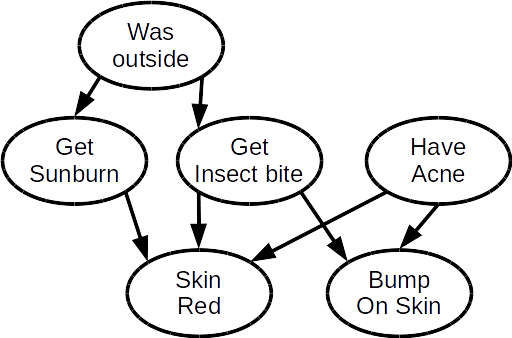
\includegraphics[width=3in]{bn.png}
\end{center}
%\vspace{0.2in}
  
The random variables are:
%
\begin{itemize}
\item \attr{Was Outside}: Was the person outside?
\item \attr{Get Sunburn}: Did the person get sunburn?
\item \attr{Get Insect Bite}: Did the person get an insect bite?
\item \attr{Have Acne}: Does the person have acne?
\item \attr{Skin Red}: Is the skin red?
\item \attr{Bump on Skin}: Is there a bump?  
\end{itemize}

\medskip
 
For the following questions, $I(A,B)$ means that events A and B are independent and $I(A,B | C)$ means that events A and B are independent conditioned on C. Use the concept of d-separation to answer the questions and show your work.

%
\begin{enumerate}
\item Is $I(\attr{Have Acne},\attr{Was Outside})$? If NO, give
intuition for why.
%
%
\item Is $I(\attr{Have Acne},\attr{Was Outside}\given \attr{Skin Red})$? If NO, give
intuition for why.
%
%
\item Is $I(\attr{Get Sunburn},\attr{Bump on Skin})$? If NO, give
intuition for why.
%
\item Is $I(\attr{Get Sunburn},\attr{Bump on Skin}\given \attr{Get Insect Bite})$? If NO, give intuition for why.
%
\item Suppose the person has taken a medicine to suppress their
  response to insect bites: they get red skin, but no bumps.  Draw the
  modified network.  
%
%
\item For this modified network, is $I(\attr{Get Sunburn},\attr{Bump
  on Skin})$? If NO, give an intuition why.  If YES, describe what
  observations (if any) would cause them to no longer be independent.    
%
\end{enumerate}
\end{problem}

\newpage

\section*{Kalman Filters [7 pts]}

\begin{problem}
  In this problem, you will implement a one-dimensional Kalman filter.
  Assume the following dynamical system model:
  \begin{eqnarray*}
    z_{t+1} &= z_{t} + \epsilon_{t} \\
    x_{t} & = z_{t} + \gamma_{t}  
  \end{eqnarray*}
  where $z$ are the hidden variables and $x$ are the observed
  measurements.  The random variables $\epsilon$ and $\gamma$ are
  drawn from the following Normal distributions:
  \begin{eqnarray*}
    \epsilon_t &\sim& N(\mueps,\sigeps) \\
    \gamma_t &\sim& N(\mugam,\siggam) 
  \end{eqnarray*}
  where $\mueps = 0$, $\sigeps=0.05$, $\mugam = 0$ and $\siggam=1.0$

  You are provided with the observed data $x$ and the hidden data $z$ in kf-data.csv, and the prior on the first hidden state is $p(z_0)$ = N($\muzp$,$\sigzp$) where $\muzp = 5$ and $\sigzp=1$


    \begin{itemize}
      \item[(a)] The distribution $p(z_t|x_0...x_t)$ will be Gaussian
        $N(\mu_t,\sigma^2_t)$. Derive an iterative update for the mean
        $\mu_t$ and variance $\sigma^2_t$ given the mean and variance
        at the previous time step ($\mu_{t-1}$ and  $\sigma^2_{t-1}$).

       \item[(b)] Implement this update and apply it to the observed data
         above (do not use the hidden data to find these updates). Provide a plot of $\mu_t$ over time as well as a
         $2\sigma_t$ interval around $\mu_t$ (that is $\mu_t \pm
         2\sigma_t$).  Does the Kalman filter ``catch up'' to the true
         hidden object?

       \item[(c)] Repeat the same process but change the observation
         at time $t=10$ to $x_{t=10}=10.2$ (an extreme outlier
         measurement).  How does the Kalman filter respond to this
         outlier?  

       \item[(d)] Comment on the misspecification of dynamical system
         model for these data.  Based on the previous two parts, how
         does this misspecification affect the predictions?

\end{itemize}    
\end{problem}

\newpage

\section*{Markov Decision Processes [7 pts]}
\begin{problem}
  ~

  
  \noindent In this problem we will explore the calculation of the \emph{MDP value function} $V$  in a 2D exploration setting, without time discounting and
for a finite time horizon. 
%
Consider a robot navigating the following grid:\\
  \begin{center}
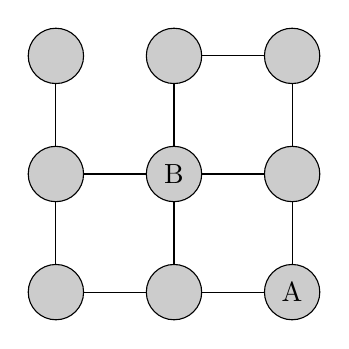
\begin{tikzpicture}[darkstyle/.style={circle,draw,fill=gray!40,minimum size=20}]
  \foreach \x in {0,...,2}
    \foreach \y in {0,...,2} 
       {\node [darkstyle]  (\x\y) at (1.5*\x,1.5*\y) {\ifthenelse{\x=2 \AND \y=0}{A}{\ifthenelse{\x=1\AND\y=1}{B}{}}};} 

       \draw (00)--(01);
       \draw (01)--(02);

       \draw (10)--(11);
       \draw (11)--(12);

       \draw (10)--(11);
       \draw (11)--(21);

       \draw (20)--(21);
       \draw (11)--(21);

       \draw (21)--(22);
       \draw (01)--(11);
       \draw (00)--(10);
       \draw (12)--(22);

       \draw (10)--(20);

\end{tikzpicture}
\end{center}
The robot moves in exactly one direction each turn (and must move). The robot's goal is to maximize its score in the game after $T$ steps. The
score is defined in the following way:
%
\begin{itemize}
  \item If the robot's movement attempts to move it off the grid, then
    the robot loses a point (-1) and stays where it is.
  \item If the robot ends its motion on node A, it receives 10 points,
    and if it moves onto node B, it receives -100 points. Otherwise, it
    receives 0 points.  
\end{itemize}

  \begin{enumerate}
    \item Model this as a Markov decision process: define the states $S$, actions $A$, reward function $r:S\times A\mapsto \mathbb{R}$, and transition model $p(s'\given s, a)$ for $s', s\in S$ and $a\in A$.  For now, assume that the robot's actions execute perfectly: if the robot tries to move in a particular direction, it always succeeds in doing so.

    \item Consider a \emph{random policy} $\pi$, where
in each state the robot moves uniformly at randomly in any of its available directions (including off the board). 
      For every position on the grid calculate the
value function, $V^\pi_t: S\mapsto 
\mathbb{R}$, under this policy, for $t=2, 1$ steps left
to go. You can find LaTeX code for the tables in the solution template. Note that you should have 2 tables, one for each time horizon. 
%
    \item Now assume that the robot plays an \emph{optimal policy}
      $\pi^\ast_t$ (for $t$ time steps to go). Find the optimal policy in the case of a finite time horizon of $t = 1, 2$ and give the corresponding 
MDP value functions $V^\ast_t: S\mapsto 
\mathbb{R}$, under this
optimal policy. You can indicate the optimal policy for each time horizon on the corresponding $V^\ast_t$ table via arrows or words in the direction that the robot should move from that state. 
    \item Now consider the situation where the robot does not have
      complete control over its movement. In particular, 
when it chooses a direction, there is a 80\% chance that it will go in
      that direction, and a 10\% chance it will go in the two adjacent
      (90$^\circ$ left or 90$^\circ$ right) 
directions. Explain how this changes the elements $S$, $A$, $r$, and $p(s' \given s,a)$ of the MDP model. 
Assume the robot uses the same
 policy $\pi^\ast_t$ from the previous question (now possibly
      non-optimal), and write this as $\pi_t$, and tie-break in favor of N, then E, then S then W.
Give the corresponding 
MDP value functions $V^\pi_t: S\mapsto 
\mathbb{R}$, for this policy in this partial control world, for $t=2, 1$ steps left
to go. Is the policy still optimal?
  \end{enumerate}
\end{problem}
%\subsection*{Solution}

%  Table starter code
%  \begin{center}
%    \begin{tabular}{c|c}
%      $s$ & $V^\pi_1(s)$ \\ \hline
%      State & 0
%    \end{tabular}
%  \end{center}

\newpage
\begin{problem}[Calibration, 1pt]
Approximately how long did this homework take you to complete?
\end{problem}


\begin{itemize}
    \item Name:
    \item Email:
    \item Collaborators:
\end{itemize}

\end{document}
